\begin{frame}[parent={cmap:software-testing-foundations}, hasprev=false, hasnext=true]
\frametitle{Teste de software}

\begin{block:fact}{Motivação}
\begin{itemize}
	\item Software contém falhas.

	\item Testar o software pode revelar várias falhas.
\end{itemize}
\end{block:fact}

\begin{block:fact}{Teste de software como uma disciplina}
\begin{itemize}
	\item Teste \textit{Ad hoc} é insuficiente e ineficaz na detecção de falhas.
	\begin{itemize}
		\item É difícil pensar em casos de testes o suficiente até mesmo para software simples.
		(como o triângulo).
	\end{itemize}

	\item O teste de software deve ser tomado como uma disciplina
	\begin{itemize}
		\item Os casos de teste devem ser criados para avaliar a qualidade dos artefatos do software (principalmente a especificação de requisitos e o código-fonte) em relação aos critérios estabelecidos.

		\item As técnicas devem ser desenvolvidas para detectar o máximo de falhas possíveis no software.
	\end{itemize}
\end{itemize}
\end{block:fact}
\end{frame}


\begin{frame}[hasprev=true, hasnext=true]
\frametitle{Teste de software}
\framesubtitle{Definição}
\label{concept:software-testing}

\begin{block:concept}{Definição}
O teste de software é o processo de operação de um sistema ou componente em condições especificadas, observando ou registrando os resultados, e fazendo uma avaliação de alguns aspectos do sistema ou componente~\cite{ieee610.12:1990}.
\end{block:concept}

\begin{block:fact}{Teste de software é\dots{}}
\begin{itemize}
	\item uma atividade de verificação e validação,

	\item importante para a manutenção, avaliação da confiabilidade, melhoria de processos de software, depuração,

	\item uma atividade dinâmica,
	\begin{itemize}
		\item Isso requer a execução do programa (análise estática não é suficiente),
	\end{itemize}

	\item custoso~\cite{harrold:2000}
\end{itemize}
\end{block:fact}
\end{frame}



\begin{frame}
\frametitle{Teste de software}
\framesubtitle{Objetivo}

\begin{block:fact}{Objetivo}
\begin{itemize}
	\item O objetivo do teste de software é detectar falhas no produto em fase de testes.
\end{itemize}
\end{block:fact}

\begin{block:fact}{}
Primeiro erro já detectado (por Grace Hopper). É um bug real (é por isso que chamamos erro de bug até hoje).
\centering
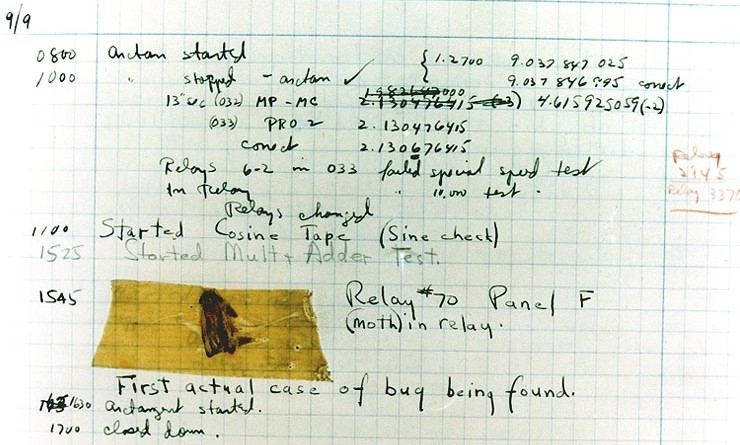
\includegraphics[width=7cm]{teste-de-software/conceitos-basicos/Imagens/first-bug}
\end{block:fact}
\end{frame}


\begin{frame}
\frametitle{Teste de software}
\framesubtitle{Análise racional}

\begin{block:fact}{Contradição}
\begin{itemize}
	\item Assim, testes de software visa apenas destruir o software?
	\begin{itemize}
		\item Afinal de contas, o programador gasta horas implementando-o e as atividades de teste encontrarão erros no trabalho feito por ele
	\end{itemize}
\end{itemize}
\end{block:fact}

\begin{block:fact}{Análise relacional}
\begin{itemize}
	\item Humans are highly goal-oriented (and proper goals has an important
	psychological effect~\cite[p. 6]{myers:2004}).

	\item Se o objetivo é demonstrar que o programa não tem nenhum erro, então o dispositivo de teste subconscientemente será conduzido em direção a esse objetivo.
	\begin{itemize}
		\item Haverá uma tendência para selecionar dados que possuem uma baixa probabilidade de causar falhas nos programas.
	\end{itemize}

	\item Se o objetivo é demonstrar que o programa tem falhas, os casos de teste terão uma maior probabilidade de encontrar os erros.
\end{itemize}
\end{block:fact}
\end{frame}



\begin{frame}
\frametitle{Teste de software}
\framesubtitle{Análise relacional}

\begin{block:principle}{Análise relacional}
O processo de demonstração de que os erros não estão presentes é impossível de alcançar virtualmente todos os programas (mesmo os triviais).
\end{block:principle}

\begin{block:fact}{Problemas indertemináveis}
\begin{itemize}
	\item A avaliação de correção de um programa é um problema indeterminável.
	\begin{itemize}
		\item Indeterminado = não computável.
	\end{itemize}

	\item Os erros podem ser camuflados por outros erros devido a correções coincidentes.
	\begin{itemize}
		\item A avaliação de correção coincidente também é um problema inderterminável.
	\end{itemize}

	\item Several other undecidable problems plague (praga, aplicáveis) software testing: software
	equivalence, executability.
\end{itemize}
\end{block:fact}
\end{frame}


\begin{frame}
\frametitle{Teste de software}
\framesubtitle{Conceitos principais}

\begin{block:fact}{Como são detectadas as falhas?}
\begin{itemize}
	\item As falhas são detectadas através da execução do software contra um conjunto de casos de teste.
\end{itemize}
\end{block:fact}

\begin{block:procedure}{Execução do caso de teste}
\begin{enumerate}
	\item Definir os dados de entrada que serão fornecidos ao software sob teste.

	\item Execute o software.

	\item Checar se os resultados das produção do software era o esperado (para os dados de entrada fornecido)
	\begin{itemize}
		\item Se o resultado é correto, mantenha a definição de diferentes casos de entrada.

		\item Se o resultado é incorreto, uma falha foi encontrada! Sucesso!
	\end{itemize}
\end{enumerate}
\end{block:procedure}
\end{frame}



\begin{frame}
\frametitle{Teste de software}
\framesubtitle{Conceitos principais}

\begin{block:principle}{Teste exaustivo}
Se o software é executado com todos os dados possíveis, qualquer falha será encontrada
\end{block:principle}

\begin{block:fact}{Viabilidade e computabilidade}
Infelizmente, muitas vezes não é possível executar testes exaustivamente devido a alguns problemas computacionais:
\begin{itemize}
	\item O dados de entrada podem ser tão grandes que é impossível executar o software com ele em um tempo razoável;

	\item Computabilidade (problemas indertemináveis).
\end{itemize}
\end{block:fact}
\end{frame}


\begin{frame}
\frametitle{Teste de software}
\framesubtitle{Conceitos principais}

\begin{block:principle}{Divisão de domínio}
No entanto, é possível particionar o domínio de entrada e, em vez de usar todos os elementos dentro de cada partição, apenas poucas entradas são selecionadas (e aceito como uma boa representação de cada elemento do conjunto).
\end{block:principle}

\begin{block:fact}{Técnicas e critérios}
\begin{itemize}
	\item Critérios de teste definem as regras a respeito de como um determinado dado de entrada é dividido;

	\item Tais regras, quando aplicado ao software sob teste, gera necessidade de teste:
	\begin{itemize}
		\item Requisitos de teste é uma combinação de elementos do programa com os testes devem ser satisfeitas pela execução de um caso de teste.
	\end{itemize}

	\item Técnicas de teste definem a razão e a fonte de informação que orienta o desenvolvimento de critérios de teste.
\end{itemize}
\end{block:fact}
\end{frame}




\begin{frame}[c, hasprev=true, hasnext=false]
\frametitle{Teste de software concepts}
\framesubtitle{Conceitos principais}

\begin{block:fact}{}
	\centering
	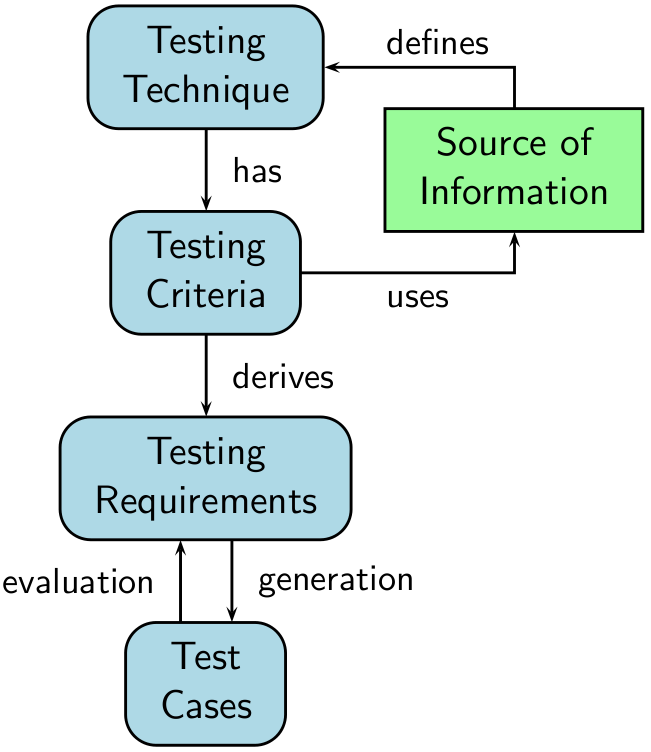
\includegraphics[scale=.3]{teste-de-software/conceitos-basicos/Imagens/software-testing}
\end{block:fact}
\end{frame}